\section{Design og implementering}\label{sec:filter_design}
For at kunne implementere anti-alias lav pas filtrene i praksis blev det valgt at designe et 
prototype print hertil. Da printet blev designet i starten af projektets forløb hvor filteret 
endnu ikke var færdig dimensioneret, blev det valgt at designe et generisk Sallen-Key biquad 
der kan anvendes til alle de fire, i litteraturen opgivet, designmetoder. Kredsløbet kan ses i 
figur \ref{fig:skbiquadsch}.



\begin{figure}[H]
	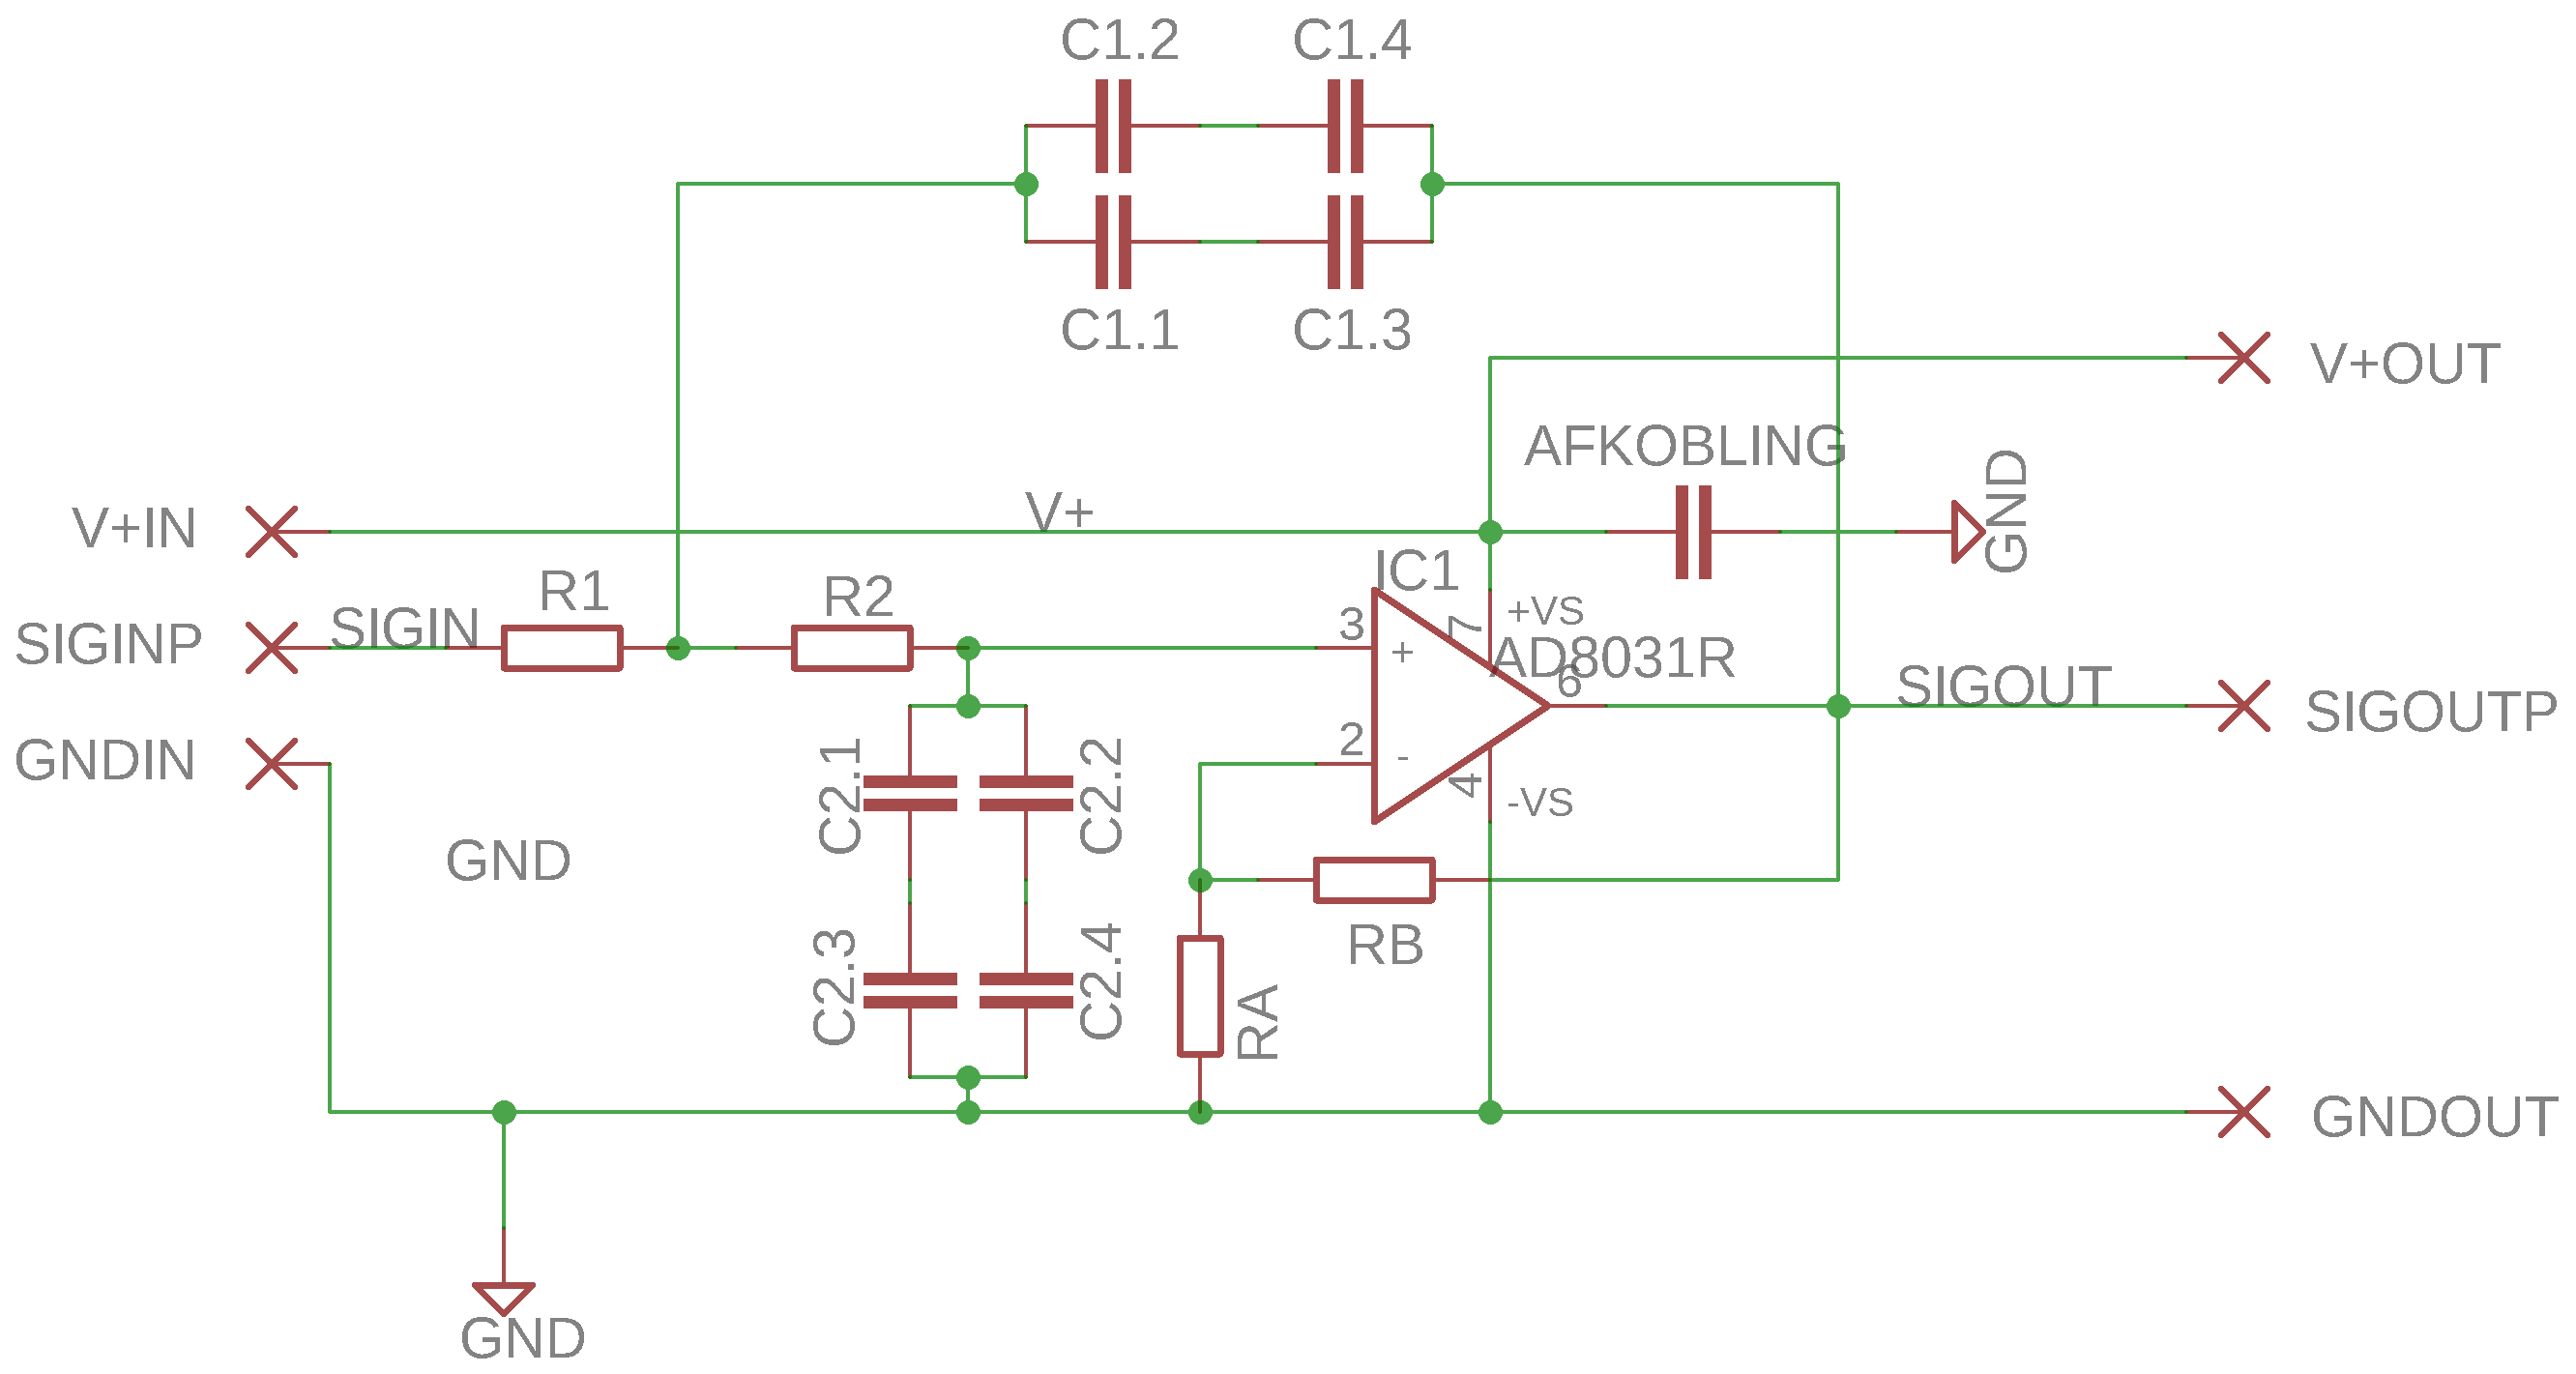
\includegraphics[width=\linewidth]{billeder/skbiquadsch}
	\caption{Lav pas biquad prototype kredsløb}
	\label{fig:skbiquadsch}
\end{figure}

Som det kan ses på figuren så er begge kondensatorer erstattet med en parallelforbindelse af 
to serie forbundne kondensatorer. Dette valg gør at det langt nemmere at opnå en specific 
kapacitans, ved at anvende op til fire kondensatorer fra rækken af værdier der er tilgængelig.

Disse kondensatorer blev beregnet ved at lave et matlab script som finder alle mulige kombinationer, for de kondensatorer som var tilgængelig på SDU under projektets udførelse.

Som det kan ses i tabel \ref{tab:kapvskap} bliver den faktiske kapacitans rigtig tæt på den
beregnede, dog er der her ikke taget højde for usikkerheden i komponentværdierne.

\begin{table}[h!]
	\centering
	\caption{Beregnede kondensatorer og tætteste mulige kombinationer serie/parallel}
	\begin{threeparttable}
		\begin{tabular}{l c c c c}
			\toprule
			& \multicolumn{2}{c}{\textbf{Beregnede værdier}} & \multicolumn{2}{c}{\textbf{Tætteste mulige kombinationer}} \\ 
			\midrule
			\textbf{Filter \#} &
			\textbf{$C_{1}$} 	& 
			\textbf{$C_{2}$}  	&
			\textbf{$C_{1}$} 		& 
			\textbf{$C_{2}$} 	\\
			\midrule
			1 & \num{2.2573E-09}\farad & \num{1,5703E-09}\farad & \num{2.2585e-09}\farad & \num{1.57e-09}\farad \\
			
			2 & \num{3,0832E-09}\farad & \num{4,3476E-10}\farad & \num{3.08073e-09}\farad & \num{4.3477e-10}\farad \\
			
			3 & \num{8,4273E-09}\farad & \num{9,8146E-11}\farad & \num{8.4259e-09}\farad & \num{9.8409e-11}\farad \\
			\bottomrule
		\end{tabular}
	\end{threeparttable}
\label{tab:kapvskap}
\end{table}

Det valgtes at lave hver bi-quad som et separat print der kan kobles sammen med et lignende
sig selv. 
Dette giver de fordele at det vil forekomme nemmere at fejlfinde på de enkelte led, og
samtidigt kan der laves flere forskellige ordener af filtret uden at skulle ændre på PCB designet.

Det færdige PCB design kan ses på figur \ref{fig:skbiquadpcb}. Her kortsluttes RB, og RA forbliver ikke forbundet, og så påsættes der selvfølgelig de beregnede komponenter for at opnå det specificerede filter bi-quad. Vis man sammenligner resultaterne fra testen i bilag 
\ref{sec:test_aafilter} med den beregnede filter karakteristik vist i figur 
\ref{fig:filter_cheb1_denorm}, kan det ses at filteret i pasbåndet har en konstant dæmpning
på ca. $3\si\decibel$. \hlh{Hvorfor er der nu den konstante dæmpning?}
Dette kan der dog ses bort fra da dæmpningen er konstant. Udover dette kan det ellers
konkluderes at implementeringen af filteret overholder designet,
da både knækfrekvensen og hældningen i mellem pas og stop bånd stemmer overens.


\begin{figure}[H]
	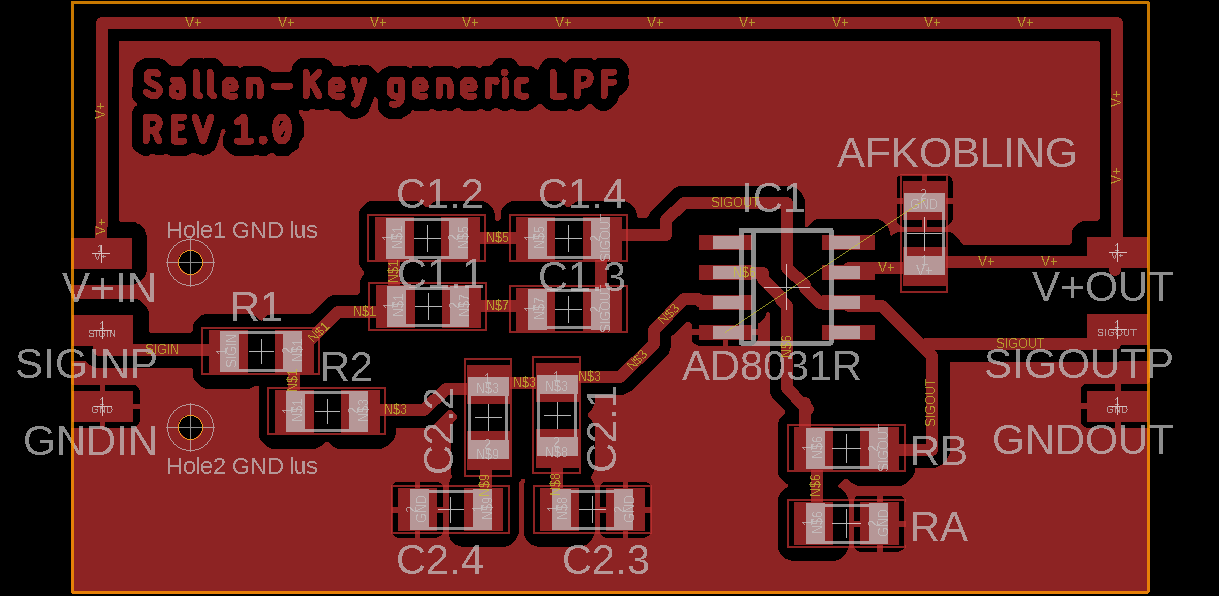
\includegraphics[width=\linewidth]{billeder/skbiquadpcb}
	\caption{Lav pas biquad prototype PCB design}
	\label{fig:skbiquadpcb}
\end{figure}
\section{Rekonstruktions filter}
\note{Hvorfor anvendes et tilsvarende AA filter på udgangen - lidt teori her}

Da udgangen fra DAC'en 
\begin{figure}[H]
	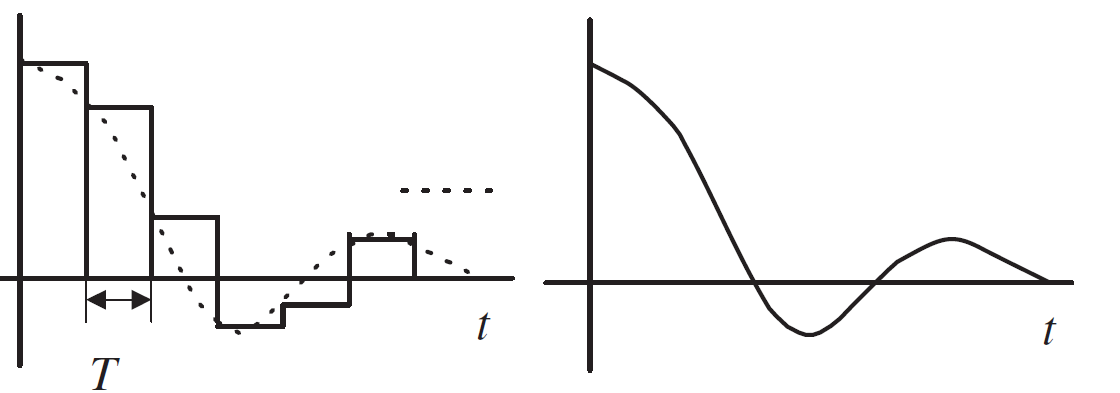
\includegraphics[width=\linewidth]{billeder/dacrecon}
	\caption{Udgang fra DAC med sample-and-hold, før og efter reconstructionsfilter. Kilde:\cite{Tan2013}}
	\label{fig:skbiquadpcb}
\end{figure}
